\section{对偶理论}
\subsection{LP 对偶问题的形式}
\begin{note}
    \figref{fig2}中,左边是对偶问题 (D),右边是原问题 (P)。
    \begin{figure}[htbp]
        \centering
        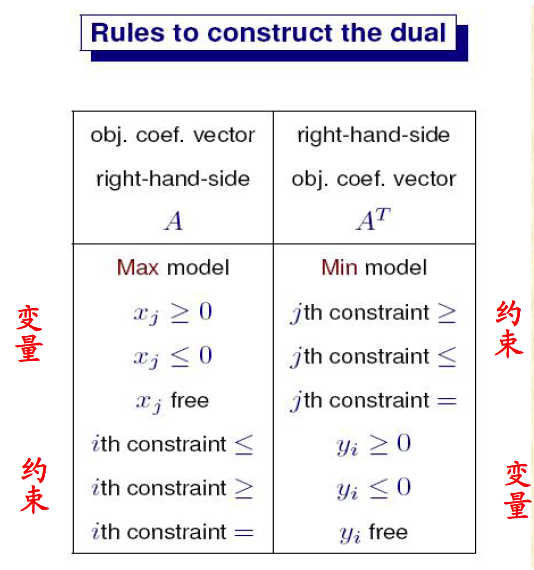
\includegraphics[width=0.4\textwidth]{./figures/img2.png}
        \caption{LP 问题的对偶问题转换规则 \label{fig2}}
    \end{figure}
    \[\begin{cases}
        \min \quad & 2x_1 + x_2 + 2x_3\\
        s.t. \quad & x_1 + x_2 + 2x_3 \ge 1\\
        &x_1 - x_2 + x_3 \le 2\\
        &-x_1 + x_2 + x_3 = 1\\
        &x_1 \ge 0, x_2 \ \text{free}, x_3 \le 0
    \end{cases} \Longrightarrow \begin{cases}
        \max \quad & w_1 + 2w_2 + w_3\\
        s.t. \quad & w_1 + w_2 - w_3 \le 2\\
        &w_1 - w_2 + w_3 = 1\\
        &2w_1 + w_2 + w_3 \ge 2\\
        &w_1 \ge 0, w_2 \le 0, w_3 \ \text{free}
    \end{cases}\]
    \begin{itemize}
        \item 原问题的变量对应对偶问题的约束,并且\textbf{符号改变}。
        \item 原问题的约束对应对偶问题的变量,符号保持,等号对应 free。
    \end{itemize}
\end{note}

\subsection{对偶问题的基本性质}
\begin{minipage}[c]{15em}
    \[
        \text{原问题 (P)}
        \begin{cases}
            \min \quad &c^tx\\
            \subject \quad &Ax \ge b\\
            &x \ge 0
        \end{cases}
    \]
\end{minipage}
\begin{minipage}[c]{15em}
    \[
        \text{对偶问题 (D)}
        \begin{cases}
            \max \quad &b^tw\\
            \subject \quad &A^tw \le c\\
            &w \ge 0
        \end{cases}
    \]
\end{minipage}

\begin{theorem}[弱对偶定理]
    弱对偶定理:若 $x^{(0)}, w^{(0)}$ 分别是原问题 (P) 和对偶问题 (D) 的可行解,则 $c^Tx^{(0)} \ge b^Tw^{(0)}$,即最小化目标的函数值大于等于最大化目标的函数值。
\end{theorem}

\begin{theorem}[弱对偶推论]
    若问题 (P) 或 (D) 有无界解,则其对偶问题 (D) 或 (P) 无可行解。
\end{theorem}

\begin{theorem}[最优性准则]
    若 $x^{(0)}$,$w^{(0)}$ 分别为 (P),(D) 的可行解且 $c^tx^{(0)} = b^tw^{(0)}$,则 $x^{(0)}$,$w^{(0)}$ 分别为 (P),(D) 问题的最优解。
\end{theorem}

\begin{theorem}[强对偶定理]
    若原问题 (P) 和对偶问题 (D) 均有可行解,则原问题 (P) 和对偶问题 (D) 均有最优解,且 (P) 和 (D) 的最优目标函数值相等。\begin{itemize}
        \item 推论:若问题 (P) 或 (D) 无可行解,则其对偶问题 (D) 或 (P) 或者无可行解,或者目标函数值趋于无穷。
        \item 推论:在用单纯形法求解 LP 问题 (P) 的松弛变量的检验数的相反数为对偶问题 (D) 的最优解。
        \item 推论:在用单纯形法求解 LP 问题 (D) 的松弛变量的检验数的为原问题 (P) 的最优解。
    \end{itemize}
\end{theorem}

\begin{example}
    求下列问题对偶问题的最优解
    \[
        \begin{cases}
            \max \quad &2x_1 + 3x_2\\
            \subject \quad &x_1 + 2x_2 \le 8\\
            &4x_1 \le 16\\
            &4x_2 \le 12\\
            &x_1, x_2 \ge 0
        \end{cases}    
    \]

    \answer
    化为标准形
    \[
        \begin{cases}
            \max \quad &2x_1 + 3x_2\\
            \subject \quad &x_1 + 2x_2 + x_3 = 8\\
            &4x_1 + x_4 = 16\\
            &4x_2 + x_5 = 12\\
            &x_1, x_2, x_3, x_4, x_5 \ge 0
        \end{cases}    
    \]

    \begin{center}
        \begin{tabular}{c|ccccc|c}
            & $x_1$ & $x_2$ & $x_3$ & $x_4$ & $x_5$ & \\
            \hline
            $x_3$ & 1 & 2 & 1 & 0 & 0 & 8\\
            $x_4$ & 4 & 0 & 0 & 1 & 0 & 16\\
            $x_5$ & 0 & {\color{red} 4} & 0 & 0 & 1 & 12\\
            \hline
            & -2 & -3 & 0 & 0 & 0 & 0
        \end{tabular}

        \begin{tabular}{c|ccccc|c}
            & $x_1$ & $x_2$ & $x_3$ & $x_4$ & $x_5$ & \\
            \hline
            $x_3$ & {\color{red} 1} & 0 & 1 & 0 & -1/2 & 2\\
            $x_4$ & 4 & 0 & 0 & 1 & 0 & 16\\
            $x_2$ & 0 & 1 & 0 & 0 & 1/4 & 3\\
            \hline
            & -2 & 0 & 0 & 0 & 3/4 & 9
        \end{tabular}

        \begin{tabular}{c|ccccc|c}
            & $x_1$ & $x_2$ & $x_3$ & $x_4$ & $x_5$ & \\
            \hline
            $x_1$ & 1 & 0 & 1 & 0 & -1/2 & 2\\
            $x_4$ & 0 & 0 & -4 & 1 & {\color{red} 2} & 8\\
            $x_2$ & 0 & 1 & 0 & 0 & 1/4 & 3\\
            \hline
            & 0 & 0 & 2 & 0 & -1/4 & 13
        \end{tabular}

        \begin{tabular}{c|ccccc|c}
            & $x_1$ & $x_2$ & $x_3$ & $x_4$ & $x_5$ & \\
            \hline
            $x_1$ & 1 & 0 & 0 & 1/4 & 0 & 4\\
            $x_5$ & 0 & 0 & -2 & 1/2 & 1 & 4\\
            $x_2$ & 0 & 1 & 1/2 & -1/8 & 0 & 2\\
            \hline
            & 0 & 0 & 3/2 & 1/8 & 0 & 14
        \end{tabular}
    \end{center}
    此时获得最优解为 $x^* = (4, 2)^t$,$maxZ = 14$。

    那么对偶问题的最优解为 $x^* = (\frac{3}{2}, \frac{1}{8}, 0)^t$,$minZ = 14$。
\end{example}

\begin{theorem}[互补松弛定理]
    互补松弛定理:设 $x^{(0)}, w^{(0)}$ 分别是 (P), (D) 问题的可行解,则 $x^{(0)},w^{(0)}$ 分别为 (P), (D) 的最优解的充要条件是 $\forall i, j (1 \le i \le m, 1\le j \le n)$ 有 \begin{itemize}
        \item 若 $x_j^{(0)} > 0$,则 $w^{(0)}P_j = c_j$
        \item 若 $w^{(0)}P_j < c_j$,则 $x_j^{(0)} = 0$
        \item 若 $w_i^{(0)} > 0$,则 $A_ix^{(0)} = b_i$
        \item 若 $A_ix^{(0)} > b_i$,则 $w_i^{(0)} = 0$
    \end{itemize}
    即 $\begin{cases}
        (c - w^{(0)}A)x^{(0)} = 0\\
        w^{(0)}(Ax^{(0)} - b) = 0
    \end{cases}$,其中 $P_j$ 是 $A$ 的第 $j$ 列,$A_i$ 是 $A$ 的第 $i$ 行。
\end{theorem}

\begin{theorem}[互补松弛定理非对称形式]
    \text{}

    设 $x^{(0)}$ 和 $w^{(0)}$ 分别是 $\begin{cases}
        \min \quad & c^tx \\
        \subject \quad & Ax = b\\
        &x \ge 0
    \end{cases}$ 和 $\begin{cases}
        \max \quad & b^tw \\
        \subject \quad & A^tw \le c
    \end{cases}$ 的可行解,则 $x^{(0)}$ 和 $w^{(0)}$ 是最优解的充要条件是 $\forall j$ \begin{itemize}
        \item $x_j^{(0)} > 0 \Longrightarrow w^{(0)}P_j = c_j$
        \item $w^{(0)}P_j < c_j \Longrightarrow x_j^{(0)} = 0$
    \end{itemize}
\end{theorem}

\begin{example}
    考虑下面问题

    \begin{minipage}[c]{0.45\linewidth}
        \[
            \text{(P)}
            \begin{cases}
                \max \quad &x_1 + 2x_2 + 3x_3 + 4x_4\\
                \subject \quad &x_1 + 2x_2 + 2x_3 + 3x_4 \le 20\\
                &2x_1 + x_2 + 3x_3 + 2x_4 \le 20\\
                &x_1, x_2, x_3, x_4 \ge 0
            \end{cases}    
        \]
    \end{minipage}
    \begin{minipage}[c]{0.45\linewidth}
        \[
            \text{(D)}
            \begin{cases}
                \min \quad &20y_1 + 20y_2\\
                \subject \quad &y_1 + 2y_2 \ge 1\\
                &2y_1 + y_2 \ge 2\\
                &2y_1 + 3y_2 \ge 3\\
                &3y_1 + 2y_2 \ge 4\\
                &y_1, y_2 \ge 0
            \end{cases}
        \]
    \end{minipage}

    己知 (D) 的最优解为 $y^* = \left(\frac{6}{5}, \frac{1}{5}\right)^t$,用互补松弛定理求出 (P) 的最优解。

    \answer
    \[
        \begin{cases}
            x_1 + 2x_2 + 2x_3 + 3x_4 = 20\\
            2x_1 + x_2 + 3x_3 + 2x_4 = 20\\
            x_1 = 0, x_2 = 0, x_3 > 0, x_4 > 0
        \end{cases}    
    \]
    解得 $x^* = (0, 0, 4, 4)^t$,$minZ = maxZ = 28$。
\end{example}

\subsection{对偶问题的经济解释}
\subsection{对偶单纯形法}
\begin{note}
    对偶单纯形法步骤 (\textbf{找的两次都要小于 0,和单纯形两次都要大于 0 相反}):
    \begin{enumerate}
        \item 化标准型,建立初始单纯形表
        \item 判断,若 $B^{-1}b \ge 0$,则已得到最优解
        \item 换基迭代 \begin{enumerate}
            \item 确定换出变量,$\bar{b_r} = \min_i\left\{\bar{b_i}\right\} < 0, x_r$ 为换出变量
            \item 确定换入变量,$\min_{j}\left\{\frac{z_j - c_j}{y_{rj}}\ |\ y_{rj} < 0\right\} = \frac{z_k - c_k}{y_{rk}}$,$x_k$ 为换入变量(若所有 $y_{rj} \ge 0$,则该 LP 问题无可行解)
            \item 换基迭代,$y_{rk}$ 为主元
        \end{enumerate}
        \item 回到第 2 步
    \end{enumerate}
\end{note}

\begin{note}
    对偶单纯形法与原单纯形法的区别:
    \begin{itemize}
        \item 原单纯形法保持原问题的可行性,对偶单纯形法保持所有检验数 $wP_j - c_j \le 0$,即保持对偶问题的可行性。
        \item 特点:先选择出基变量,再选择进基变量。
    \end{itemize}
\end{note}

\begin{example}
    用对偶单纯形法求解
    \[
        \begin{cases}
            \min \quad &x_1 + x_2 + x_3\\
            \subject \quad &3x_1 + x_2 + x_3 \ge 1\\
            &-x_1 + 4x_2 + x_3 \ge 2\\
            &x_1, x_2, x_3 \ge 0
        \end{cases}    
    \]

    \answer 引入松弛变量,化为标准形
    \[
        \begin{cases}
            \min \quad &x_1 + x_2 + x_3\\
            \subject \quad &-3x_1 - x_2 - x_3 + x_4 = -1\\
            &x_1 - 4x_2 - x_3 + x_5 = -2\\
            &x_1, x_2, x_3, x_4, x_5 \ge 0
        \end{cases}    
    \]

    \begin{center}
        \begin{tabular}{c|ccccc|c}
            & $x_1$ & $x_2$ & $x_3$ & $x_4$ & $x_5$ & \\
            \hline
            $x_4$ & -3 & -1 & -1 & 1 & 0 & -1\\
            $x_5$ & 1 & {\color{red} -4} & -1 & 0 & 1 & -2\\
            \hline 
            & -1 & -1 & -1 & 0 & 0 & 0
        \end{tabular}

        \begin{tabular}{c|ccccc|c}
            & $x_1$ & $x_2$ & $x_3$ & $x_4$ & $x_5$ & \\
            \hline
            $x_4$ & {\color{red} -13/4} & 0 & -3/4 & 1 & -1/4 & -1/2\\
            $x_2$ & -1/4 & 1 & 1/4 & 0 & -1/4 & 1/2\\
            \hline 
            & -5/4 & 0 & -3/4 & 0 & -1/4 & 1/2
        \end{tabular}

        \begin{tabular}{c|ccccc|c}
            & $x_1$ & $x_2$ & $x_3$ & $x_4$ & $x_5$ & \\
            \hline
            $x_1$ & 1 & 0 & 3/13 & -4/13 & 1/13 & 2/13\\
            $x_2$ & 0 & 1 & 4/13 & -1/13 & -3/13 & 7/13\\
            \hline 
            & 0 & 0 & -6/13 & -5/13 & -2/13 & 9/13
        \end{tabular}
    \end{center}
    故 $x^* = (\frac{2}{13}, \frac{7}{13}, 0, 0, 0)^t$ 是最优解,$f_{\min} = \frac{9}{13}$,对偶问题的最优解是 $(\frac{5}{13}, \frac{2}{13})^t$。
\end{example}

\begin{note}
    (对偶)单纯形法步骤总结
    \begin{itemize}
        \item 单纯形法求解最小值问题,第一步找最大的判别数,第二步找最小的比值(分母大于零)
        \item 单纯形法求解最大值问题,第一步找最小的判别数,第二步找最小的比值(分母大于零)
        \item 对偶单纯形法求解最小值问题,第一步找最小的 $B^{-1}b$,第二步找最小的比值(分母小于零)
    \end{itemize}    
\end{note}

\subsection{原 - 对偶算法}
原 - 对偶算法不考。